% !TEX TS-program = xelatex
% !TEX encoding = UTF-8 Unicode 

% \documentclass[AutoFakeBold]{LZUThesis}
\documentclass[AutoFakeBold]{LZUThesis}
\usepackage{multirow}
\usepackage{threeparttable}
\CTEXsetup[name={第,部分}]{chapter}
\lstset{
language = MATLAB,
backgroundcolor=\color{white},   % choose the background color; you must add \usepackage{color} or \usepackage{xcolor}  
basicstyle=\footnotesize,        % the size of the fonts that are used for the code  
breakatwhitespace=false,         % sets if automatic breaks should only happen at whitespace  
breaklines=true,                 % sets automatic line breaking  
captionpos=bl,                    % sets the caption-position to bottom  
% commentstyle=\color{green},    % comment style  
% deletekeywords={...},            % if you want to delete keywords from the given language  
% escapeinside={\%*}{*)},          % if you want to add LaTeX within your code  
extendedchars=true,              % lets you use non-ASCII characters; for 8-bits encodings only, does not work with UTF-8  
frame=shadowbox,                    % adds a frame around the code  
keepspaces=true,                 % keeps spaces in text, useful for keeping indentation of code (possibly needs columns=flexible)  
keywordstyle=\color{blue},       % keyword style  
% language=Python,                 % the language of the code  
morekeywords={*,...},            % if you want to add more keywords to the set  
numbers=left,                    % where to put the line-numbers; possible values are (none, left, right)  
numbersep=5pt,                   % how far the line-numbers are from the code  
numberstyle=\tiny\color{gray}, % the style that is used for the line-numbers  
rulecolor=\color{black},         % if not set, the frame-color may be changed on line-breaks within not-black text (e.g. comments (green here))  
showspaces=false,                % show spaces everywhere adding particular underscores; it overrides 'showstringspaces'  
showstringspaces=false,          % underline spaces within strings only  
showtabs=false,                  % show tabs within strings adding particular underscores  
stepnumber=1,                    % the step between two line-numbers. If it's 1, each line will be numbered  
stringstyle=\color{orange},     % string literal style  
tabsize=2,                       % sets default tabsize to 2 spaces  
% title=signalAnalysis.m           % show the filename of files included with \lstinputlisting; also try caption instead of title  
}  

\begin{document}
%=====%
%
%封皮页填写内容
%
%=====%

% 标题样式 使用 \title{{}}; 使用时必须保证至少两个外侧括号
%  如: 短标题 \title{{第一行}},  
% 	      长标题 \title{{第一行}{第二行}}
%             超长标题\tiitle{{第一行}{...}{第N行}}

\title{{物联网:一项调查}}



% 标题样式 使用 \entitle{{}}; 使用时必须保证至少两个外侧括号
%  如: 短标题 \entitle{{First row}},  
% 	      长标题 \entitle{{First row}{ Second row}}
%             超长标题\entitle{{First row}{...}{ Next N row}}
% 注意:  英文标题多行时 需要在开头加个空格 防止摘要标题处英语单词粘连.

\author{\CJKfontspec{楷体}李文涛}
\major{电子信息基地班}
\college{320200928101}
\grade{2020级}



\maketitle
\frontmatter

%中文摘要
\ZhAbstract{
    本文讨论的是物联网。这种有前途的模式的主要实现因素是多种技术和通信解决方案的集成。识别和跟踪技术,有线和无线传感器和执行器网络,增强的通信协议(与下一代互联网共享),以及智能对象的分布式智能是最相关的。不难想象,任何对物联网发展的重大贡献都必须是电信、信息学、电子学和社会科学等不同知识领域协同活动的结果。在如此复杂的情况下,这项调查是针对那些想要接近这一复杂学科并为其发展做出贡献的人。报告了这种物联网范式的不同愿景,并审查了使能技术。出现的情况是,研究界仍将面临重大问题。其中最相关的是详细说明。
}
{物联网,普适计算,射频识别系统}


%英文摘要
\EnAbstract{This paper introduces the advantages and advantages of $\mathrm{HDB_3}$, 
and then uses MATLAB to program,
 complete the $\mathrm{HDB_3}$ encoding of the original digital signal sequence and the subsequent spectrum analysis of the signal, 
 and the spectral diagram visualization of the encoding time frequency domain analysis, 
 and analyze its characteristics in its transmission rate and frequency utilization.
 Finally, its application value is analyzed according to its spectral characteristics.
    \fontspec{Times New Roman}}
{Advantages and disadvantages, time frequency domain analysis, application analysis}

%生成目录
% \tableofcontents
% \addcontentsline{toc}{chapter}{目录}
% \thispagestyle{empty}


%文章主体
\mainmatter



\section{介绍}

物联网(IoT)是一种新颖的范式,在现代无线通信场景中正在迅速取得进展。这一概念的基本思想是我们周围无处不在的各种事物或物体——如射频识别(RFID)标签、传感器、执行器、移动电话等——它们通过独特的寻址方案,能够相互交互,并与它们的邻居合作,以达到共同的目标。

毫无疑问,物联网理念的主要优势在于它将对潜在用户日常生活和行为的几个方面产生巨大影响。从私人用户的角度来看,物联网引入的最明显的影响将在工作和家庭领域都可见。
在这种情况下,智能家居技术、辅助生活、电子健康、增强学习只是几个可能的应用场景的例子,在这些场景中,新范式将在不久的将来发挥主导作用。同样,从业务用户的角度来看,最明显的后果将在自动化和工业制造、物流、业务/流程管理、人员和货物的智能运输等领域同样可见。

\subsection{改进后的AMI码与$\mathrm{HDB_3}$码}

为了改进AMI码的应用能力,出现了对AMI改进后得到的几种编码方式,例如B8ZS、B6ZS、$\mathrm{HDB_3}$、B3ZS等编码方式,
其中我们对$\mathrm{HDB_3}$进行研究。

作为在欧洲E载波系统中均应用的代码,$\mathrm{HDB_3}$使用“000V”或“B00V”模式之一替换4个连续的零位。
做出选择以确保具有连续不同的极性。\cite{enwiki:1}

\section{解析计算}

数字基带信号一般是随机信号,因此不能用求确定信号频谱函数的方法来分析它的频谱特性。随机信号的频谱特性必须用功率谱密度来描述。对任意一种给定的数字基带信号,计
算功率谱密度不是一件容易的事,往往需要繁复的数学计算。
假设数字基带信号以某种标准波形$g(t)$在码元周期$ T_s $内传送出去,则数字基带信号可用随机序列
\begin{equation}
    S(t) = \sum\limits^{\infty}_{n = -\infty} a_n g(t - nT_s)
\end{equation}
表示。

通过查阅课本\cite{POCBook},$\mathrm{HDB_3}$信号的功率谱密度由下式给出:

\begin{equation}
    P_S(f) = \frac{1}{T_b} \cdot \sin^2{(\pi f T_b)} \cdot \frac{A_b^2T_b^2}{4}  \mathrm{sinc}^2{\frac{f T_b}{2}}
\end{equation}

按照要求,我们将$g(t)$的波形选为持续$1~\mu s$的矩形脉冲。

结合$\mathrm{HDB_3}$码的特性,$\{a_n\}$是零均值相关序列,
通过理论计算,我们得到下面的$\mathrm{HDB_3}$码信号的解析表达:

\begin{equation}
    P_S(f) = 2.5\times 10^{-7}\sin^2{(10^{-6}\pi f)} \mathrm{sinc}^2 (5\times 10^{-7} f)
\end{equation}

\section{代码数值计算}
\subsection{实际信号}

首先,我们通过查阅资料,$\mathrm{HDB_3}$的编码规则如本页表格所示:

% Please add the following required packages to your document preamble:
% \usepackage{multirow}
\begin{table}[]
    \begin{center}
        \begin{threeparttable}
        \begin{tabular}{|c|c|c|c|}
    \hline
    \multicolumn{1}{|r|}{自上一个v以来的+\textbackslash{}-信号数量奇偶性} & \multicolumn{1}{r|}{替换码型} & \multicolumn{1}{r|}{上一个脉冲} & \multicolumn{1}{l|}{编码} \\ \hline
    \multirow{2}{*}{偶数}                                     & \multirow{2}{*}{B00V}     & +                          & -00-                    \\ \cline{3-4} 
                                                            &                           & -                          & +00+                    \\ \hline
    \multirow{2}{*}{奇数}                                     & \multirow{2}{*}{000V}     & +                          & 000+                    \\ \cline{3-4} 
                                                            &                           & -                          & 000-                    \\ \hline
    \end{tabular}

\begin{tablenotes}
    \footnotesize
    \item \begin{center}($\mathrm{HDB_3}$编码规则示意表格)\end{center}
  \end{tablenotes}
\end{threeparttable}
\end{center}
    \end{table}


    这些规则适用于代码,因为它是从原始字符串构建的。
    每次代码中有 4 个连续的零时,它们将被替换为 000-、000+、+00+ 或 -00-。
    为了确定使用哪种模式,必须计算自最后一个违规位 V 以来的正数 (+) 和负数 (-)。如果结果是奇数,
    则使用 000− 或 000+。如果结果是偶数,则使用 +00+ 或 -00-。
    要确定使用哪种极性,必须查看四个零之前的脉冲。
    如果必须使用 000V 形式,则 V 简单地复制最后一个脉冲的极性,
    如果必须使用 B00V 形式,则选择的 B 和 V 将具有与最后一个脉冲相反的极性。

即将展示的代码采用了连续信号傅氏变换的数值计算方法\cite{ssmat},
算法的理论依据如下:
\begin{equation}
    F(j\omega)  = \int\limits_{-\infty}^{\infty} f(t) e^{-j\omega t} \mathrm{d}t =
    \lim\limits_{\tau \to 0} \sum\limits_{n = -\infty}^{n = \infty} f(n\tau) e^{-j\omega n\tau} \tau
\end{equation}

当取$\tau$足够小时,我们可以取用它的近似式,当$f(t)$为时限信号或是在$|t|$达到一定
大小时$f(t)$的衰减程度很高,则认为$n$取值有限,有:

\begin{equation}
    F(k) = \tau \sum\limits_{n = 0}^{N - 1} f(n\tau) e^{-j\omega_k n\tau} \; , \quad 0 \leq k \leq N
\end{equation}

按照此理论基础,编写了下面的代码,以对信号进行时频域分析。

\begin{lstlisting}
    %signalAnalysis.m 
    clear all;
x=[0 1 1 0 0 0 0 0 1 0 1 1 0 1 0 0 0 0 0 0 0 1 0 0 0 0 0 1 0 0 1 1 1 0 1 0 0 1 0 1];% 输入原码
y=x;% 输出y初始化
num=0;% 计数器初始化
for k=1:length(x)
   if x(k)==1
      num=num+1;                % "1"计数器
         if num/2 == fix(num/2) % 奇数个1时输出-1,进行极性交替
              y(k)=1;
         else
              y(k)=-1;
         end
    end
end
        % HDB3编码

num=0;  % 连零计数器初始化
yh=y;  % 输出初始化
sign=0; % 极性标志初始化为0
V=zeros(1,length(y));% V脉冲位置记录变量 
B=zeros(1,length(y));% B脉冲位置记录变量
for k=1:length(y)
   if y(k)==0
       num=num+1;  % 连“0”个数计数
       if num==4   % 如果4连“0”
         num=0;    % 计数器清零
         yh(k)=1*yh(k-4); 
                            % 让0000的最后一个0改变为与前一个非零符号相同极性的符号
         V(k)=yh(k);        % V脉冲位置记录
         if yh(k)==sign     % 如果当前V符号与前一个V符号的极性相同
            yh(k)=-1*yh(k); % 则让当前V符号极性反转,以满足V符号间相互极性反转要求
            yh(k-3)=yh(k);  % 添加B符号,与V符号同极性
            B(k-3)=yh(k);   % B脉冲位置记录
            V(k)=yh(k);     % V脉冲位置记录
            yh(k+1:length(y))=-1*yh(k+1:length(y));
                            % 并让后面的非零符号从V符号开始再交替变化
         end
       sign=yh(k);          % 记录前一个V符号的极性
     end
  else
      num=0;                % 当前输入为“1”则连“0”计数器清零
  end
end                         % 编码完成
qts=yh;
baudTime = 1e-6;
n = 400;
dt=baudTime/n;
% qts = [1];
T = baudTime*length(qts);
t=0:dt:T;
f=zeros(1,length(t));

for i = 1:(length(qts))
    f((i-1)*n+1:(i-1)*n+201) = qts(i);
end
N = 1024;
W1=5e6; %频率宽度
k=0:N;W=k*W1/N; %采样数为N,W为频率正半轴的采样点
ej = exp(-1j*t'*W);
F=f*ej*baudTime; %求F(jw) 
W=[-fliplr(W),W(2:N+1)]; %形成负半轴及正半轴的2N+1个频率点W
F=[fliplr(F),F(2:N+1)]; %形成对应于W的F(jw)的值
Hw = abs(F);
phi = angle(F);
Eng = F.*conj(F);
figure;
subplot(4,1,1);plot(t,f);
xlabel('t/s');ylabel('f(t)');
title('f(t)');
subplot(4,1,2);plot(W,Hw);
xlabel('f/Hz');ylabel('H(f)/V');
title('H(f)')
subplot(4,1,3);plot(W,phi);
xlabel('f/Hz');ylabel('phase/rad');
title('phase')
subplot(4,1,4);plot(W,Eng);
xlabel('f/Hz');ylabel('W/J');
title('Enegy')
\end{lstlisting}

通过运行代码输出图1.1中的时频域分析:

\begin{figure}[htbp]
    \centering
    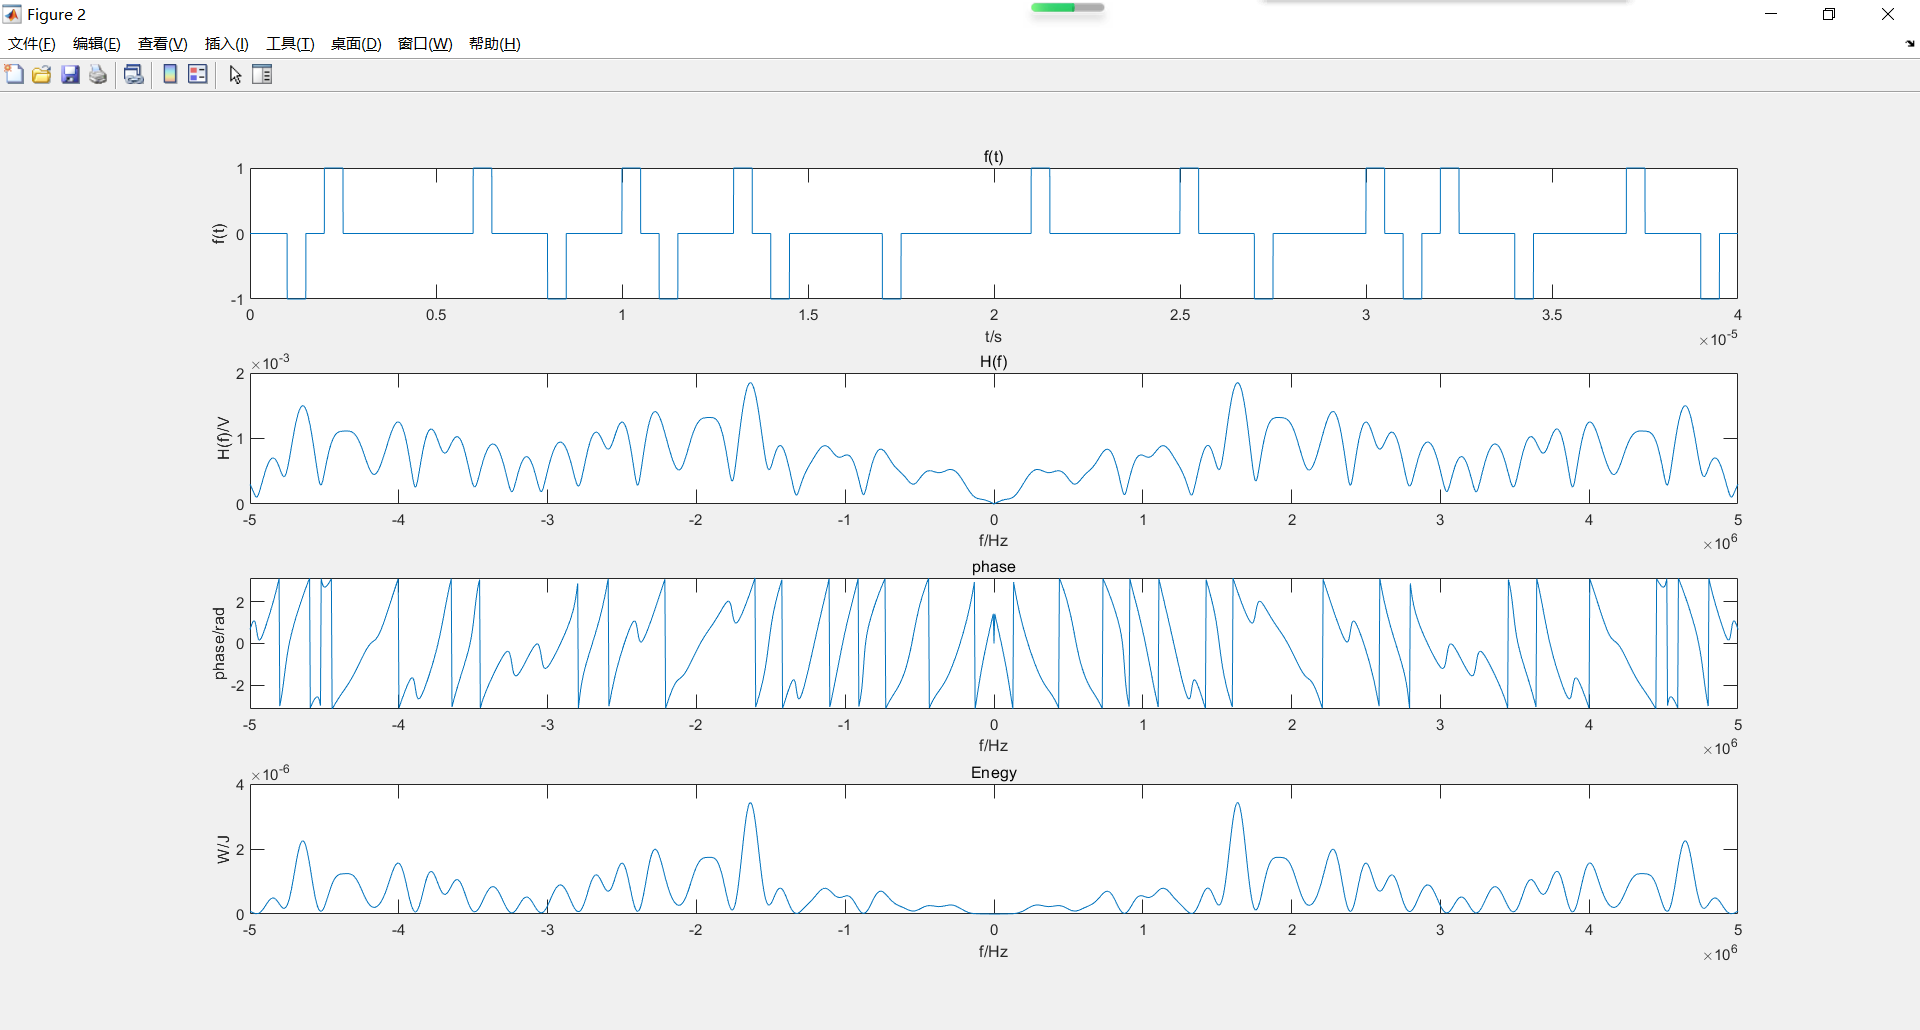
\includegraphics[keepaspectratio,width=360pt]{HDB3.png}
    \caption{实际时限信号时频域分析图}
\end{figure}

\newpage

\subsection{理想随机信号}
取消上面代码中第49行的注释,将输入信号置为理想信号,利用$plot$函数绘出此功率谱。

同样运行代码,得到图1.2中的频谱。

\begin{figure}[htbp]
    \centering
    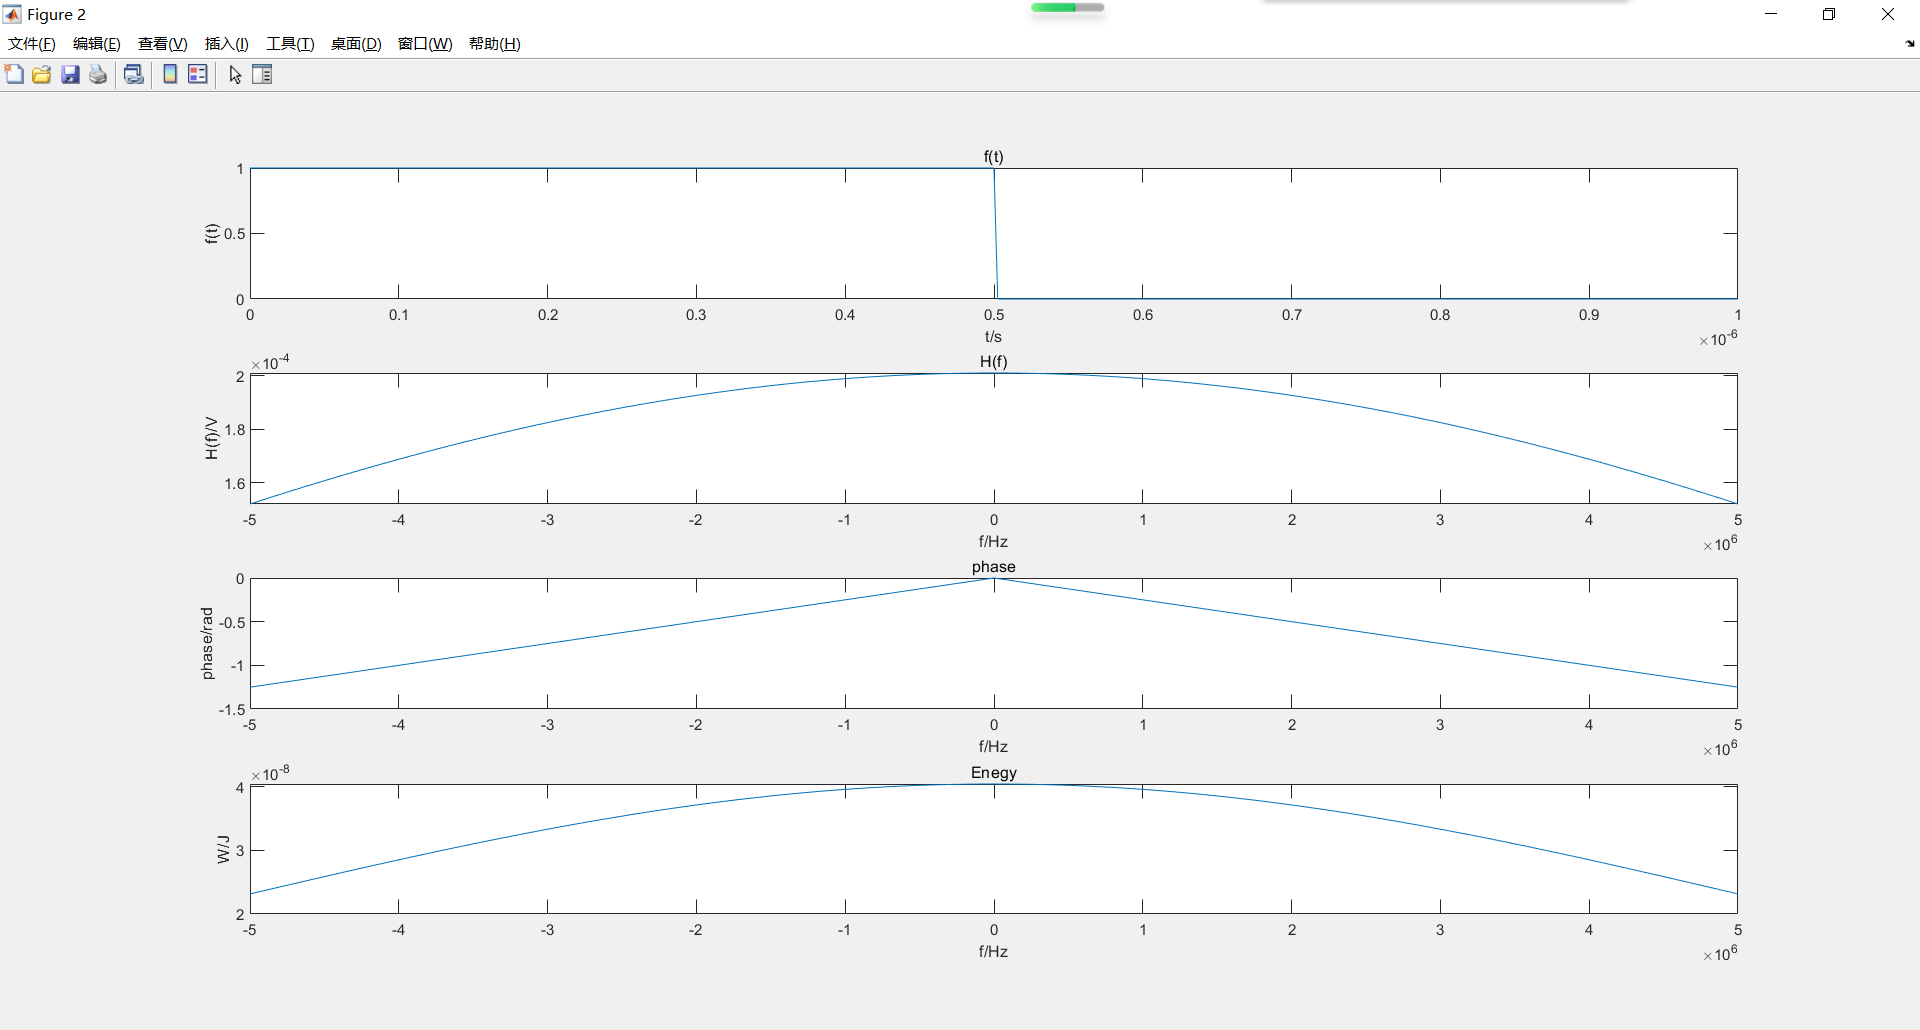
\includegraphics[keepaspectratio,width=360pt]{HDB3IM.png}
    \caption{理想随机信号时频域分析图}
\end{figure}

\chapter{计算结果分析}

\section{仿真数据分析}

\subsection{时域分布}
$\mathrm{HDB_3}$码作为改良过后的AMI码,信号中不含直流分量,
含有长连0信号的$\mathrm{HDB_3}$的编码波形在连零时仍呈现正负交替
现象,与AMI编码时信号长电平时间不跳变形成对比。
这种信号具有能量分散,抗破坏性强的特点。

\subsection{频域分布}
    由图可见$\mathrm{HDB_3}$码的功率谱低频分量较少,具有丰富的高频分量,
    具有较高的频带利用率,传输时在速度上更具优势,
    不易造成群时延失真,但会出现码间干扰,
    在进行传输时,高频分量较多的$\mathrm{HDB_3}$码可以传输更远的距离。

\section{优缺点分析}
同AMI一样,$\mathrm{HDB_3}$码正负脉冲平均电压为零,直流分量较少。
在信号到达解码电路之前,可以方便、廉价地去除直流分量。\cite{enwiki:2}

较AMI码来说,$\mathrm{HDB_3}$码的错误检测更具有优势,
在需要频繁转换的情况下,$\mathrm{HDB_3}$码能够缓解AMI码的缺陷。
能够实现更好的多路复用。

相较于归零码来说,$\mathrm{HDB_3}$中的脉冲能量不及NRZ码,但不需要与信号一起发送的单独的时钟。
但与不归零格式相比,需要使用两倍的带宽来实现相同的数据速率。

$\mathrm{HDB_3}$尽管归零包含同步的规定,但它仍然可能具有直流分量,
导致在0 或 1 位的长字符串期间出现基线漂移,就像线路代码不归零一样。



\backmatter


% %=======%
% %引入参考文献文件
% %=======%
\bibdatabase{bib/POC}%bib文件名称 仅修改bib/ 后部分
\printbib
\nocite{*} %显示数据库中有的,但是正文没有引用的文献


% \Appendix

% 这里是附录页,可要可不要

% \Thanks.



\end{document}